% !TEX TS-program = xelatex
% !BIB TS-program = bibtex
\documentclass[12pt,letterpaper]{article}
\usepackage{style/dsc180reportstyle} % import dsc180reportstyle.sty
\usepackage{hyperref}

%%%%%%%%%%%%%%%%%%%%%%%%%%%%%%%%%%%%%%%%%%%%%%%%%%%%%%%%
%%%% Title and Authors
%%%%%%%%%%%%%%%%%%%%%%%%%%%%%%%%%%%%%%%%%%%%%%%%%%%%%%%%

\title{Drone Degradation Control Adaptation through Proximal Policy Optimization}

\author{Jacob Doan \\
  {\tt j5doan@ucsd.edu} \\\And
  Bryan Zhang \\
  {\tt brzhang@ucsd.edu} \\\And
  Yi-Hsuan Kuo \\
  {\tt y3kuo@ucsd.edu} \\\And
  Jeremy Cho \\
  {\tt jec056@ucsd.edu} \\\And
  Tauhidur Rahman \\
  {\tt trahman@ucsd.edu} \\}

\begin{document}
\maketitle

%%%%%%%%%%%%%%%%%%%%%%%%%%%%%%%%%%%%%%%%%%%%%%%%%%%%%%%%
%%%% Abstract and Links
%%%%%%%%%%%%%%%%%%%%%%%%%%%%%%%%%%%%%%%%%%%%%%%%%%%%%%%%

\begin{abstract}
    Quadrotors can lose motor performance during flight, for example when a worn motor suddenly produces less thrust than commanded. A controller that adapts to such a fault could keep the drone flying long enough to finish its task or land safely, instead of crashing or abandoning the mission. Classical fault-tolerant controllers often assume the fault has already been detected and identified, and vision-aided methods estimate the drone's state from onboard cameras after a failure. Learning-based controllers can instead infer a fault from flight data without being told about it, but it remains unclear when a learned correction actually improves on a well-tuned classical controller, and how much recent flight history it needs. We study these questions in simulation with a quadrotor that follows random but repeatable curved paths between a start and a goal point, while one randomly chosen motor suddenly loses 10 to 50\% of its thrust partway through the flight. On identical flights we compare four controllers: a PID controller alone; the PID plus a correction learned with reinforcement learning (proximal policy optimization, PPO); the same correction given a window of recent states; and a PPO policy that sets the motor thrusts directly, without a PID. The learned controllers see only what a real drone would know in flight (its position and motion relative to the target, noisy IMU readings (accelerometer and gyroscope), and its last motor commands) and are never told which motor failed, when, or how badly. We rank controllers by crash rate, final distance to the goal, and recovery time, and separate controller failures from faults that no controller could survive. Finally, we remove inputs and vary the history length to find which data matter most.
\end{abstract}

\begin{center}
Code: \url{https://github.com/j2doan/drone-degradation-control}
\clearpage
\end{center}

\maketoc
\clearpage

%%%%%%%%%%%%%%%%%%%%%%%%%%%%%%%%%%%%%%%%%%%%%%%%%%%%%%%%
%%%% Main Contents
%%%%%%%%%%%%%%%%%%%%%%%%%%%%%%%%%%%%%%%%%%%%%%%%%%%%%%%%

\section{Introduction}

Quadrotors depend on coordinated thrust from four motors to maintain stable flight and follow a desired trajectory. However, motor or propeller degradation can reduce the thrust produced by a given command, introducing an imbalance that the flight controller must compensate for. If the flight controller cannot compensate for this loss of performance quickly enough, the resulting loss of control may lead to a crash. Controllers that tolerate such changes could improve flight reliability when physical repair is unavailable. This study will focus on abrupt, partial thrust loss in a single motor during path following. Reinforcement learning (RL) is a natural tool for this, since an RL policy can learn from flight data to compensate for a fault it is never explicitly told about. We aim to explore three questions about a sudden partial thrust loss (10--50\%) in one motor during path following:

\begin{enumerate}
    \item When does a learned correction make a quadrotor more likely to survive than a well-tuned PID controller alone?
    \item How much recent flight history does that correction need?
    \item Can PPO alone outperform the other fault-control methods?
\end{enumerate}

Prior work has established that quadrotors can maintain flight after complete rotor failure by relinquishing yaw regulation and adopting a spinning flight regime \citep{mueller2014}. In addition, vision-based approaches have extended fault-tolerant flight to onboard state estimation using cameras, reducing reliance on external position sensing \citep{Sun_2021}. These approaches address important aspects of flight after rotor failure, including control under reduced actuation and state estimation during rapid rotation.

Learning-based approaches offer several ways to address rotor faults. Sharma et al. trained a Soft Actor-Critic policy for hovering, landing, and path following after a single rotor failure, assuming that a separate fault detector triggers takeover by the learned controller \citep{sharma2021modelfreedeepreinforcementlearning}. Chen et al. developed a hierarchical controller in which a learned selector-controller replaces the low-level control component beneath a high-level controller that includes PID position control. Their method handles single-rotor faults of varying severity without supplied fault information at deployment, although fault information is used during training \citep{chen2025learningbasedpassivefaulttolerantcontrol}. Kim et al. combined a nominal PID controller with an RL correction and a transformer-based adaptation module that processes recent state and command history. They evaluated partial thrust loss during hovering and compared their method with PID alone and a version using a convolutional adaptation module \citep{kim2025reinforcementlearningbasedfaulttolerantcontrol}. Prior work already compares a learned correction with a PID and compares history-processing architectures. However, each study proposes one learned design and evaluates it against a small set of baselines, so the individual design choices (e.g. adding a correction to the PID versus replacing it, giving the policy a history or not, and how long that history should be) are not isolated on a common set of flights and compared against each other. To our knowledge, none of them reports at which fault sizes a carefully built PID stops being sufficient, which is what determines when a learned controller is worth adding.

Damaged drones in these relevant studies have enough thrust to hover normally without crashing. A crash is therefore usually the controller's failure rather than a physical limit: the controller must push the weak motor harder and rebalance the other three to stay on course. We will adopt this approach into our study to answer our three questions. We compare four controllers on an identical, repeatable set of flights: a PID alone, the PID plus a correction learned with PPO (a residual correction), the same residual correction given a window of recent states as additional input, and a PPO policy that sets the motor thrusts directly, replacing the PID. We rank them by crash rate, then by final distance to the goal and recovery time. Unlike prior studies, comparing these controllers in pairs isolates one design choice at a time: whether a learned correction helps (PID alone vs. PID with a correction), whether recent history helps (the correction with vs. without a window of past states), and whether the PID is needed at all (the correction vs. the policy alone). Repeating the history-based controller with different window lengths then answers the second question. The learned policies see only information a real drone would have in flight (the target's position and velocity relative to the drone, the drone's own velocity, orientation and rotation rate, noisy inertial measurement unit (IMU) readings, and their own previous thrust commands), and are never told which motor failed, when, or how badly. For the third question, we can compare the performance of each control method to determine which one was the most successful under our conditions.

Because no existing dataset covers this problem, we generate our own data in simulation, which suits these questions in three ways. We can fly as many faulty flights as needed without risking a real drone. Every fault is known exactly (which motor, how much thrust it lost, and when), so each outcome can be explained even though the controllers never see the fault; and every controller flies exactly the same flights. Therefore, any difference in performance comes from the controller alone. See Figure \ref{fig:sim-example} for a visual example of a simulated baseline flight.

\begin{figure}[H]
    \centering
    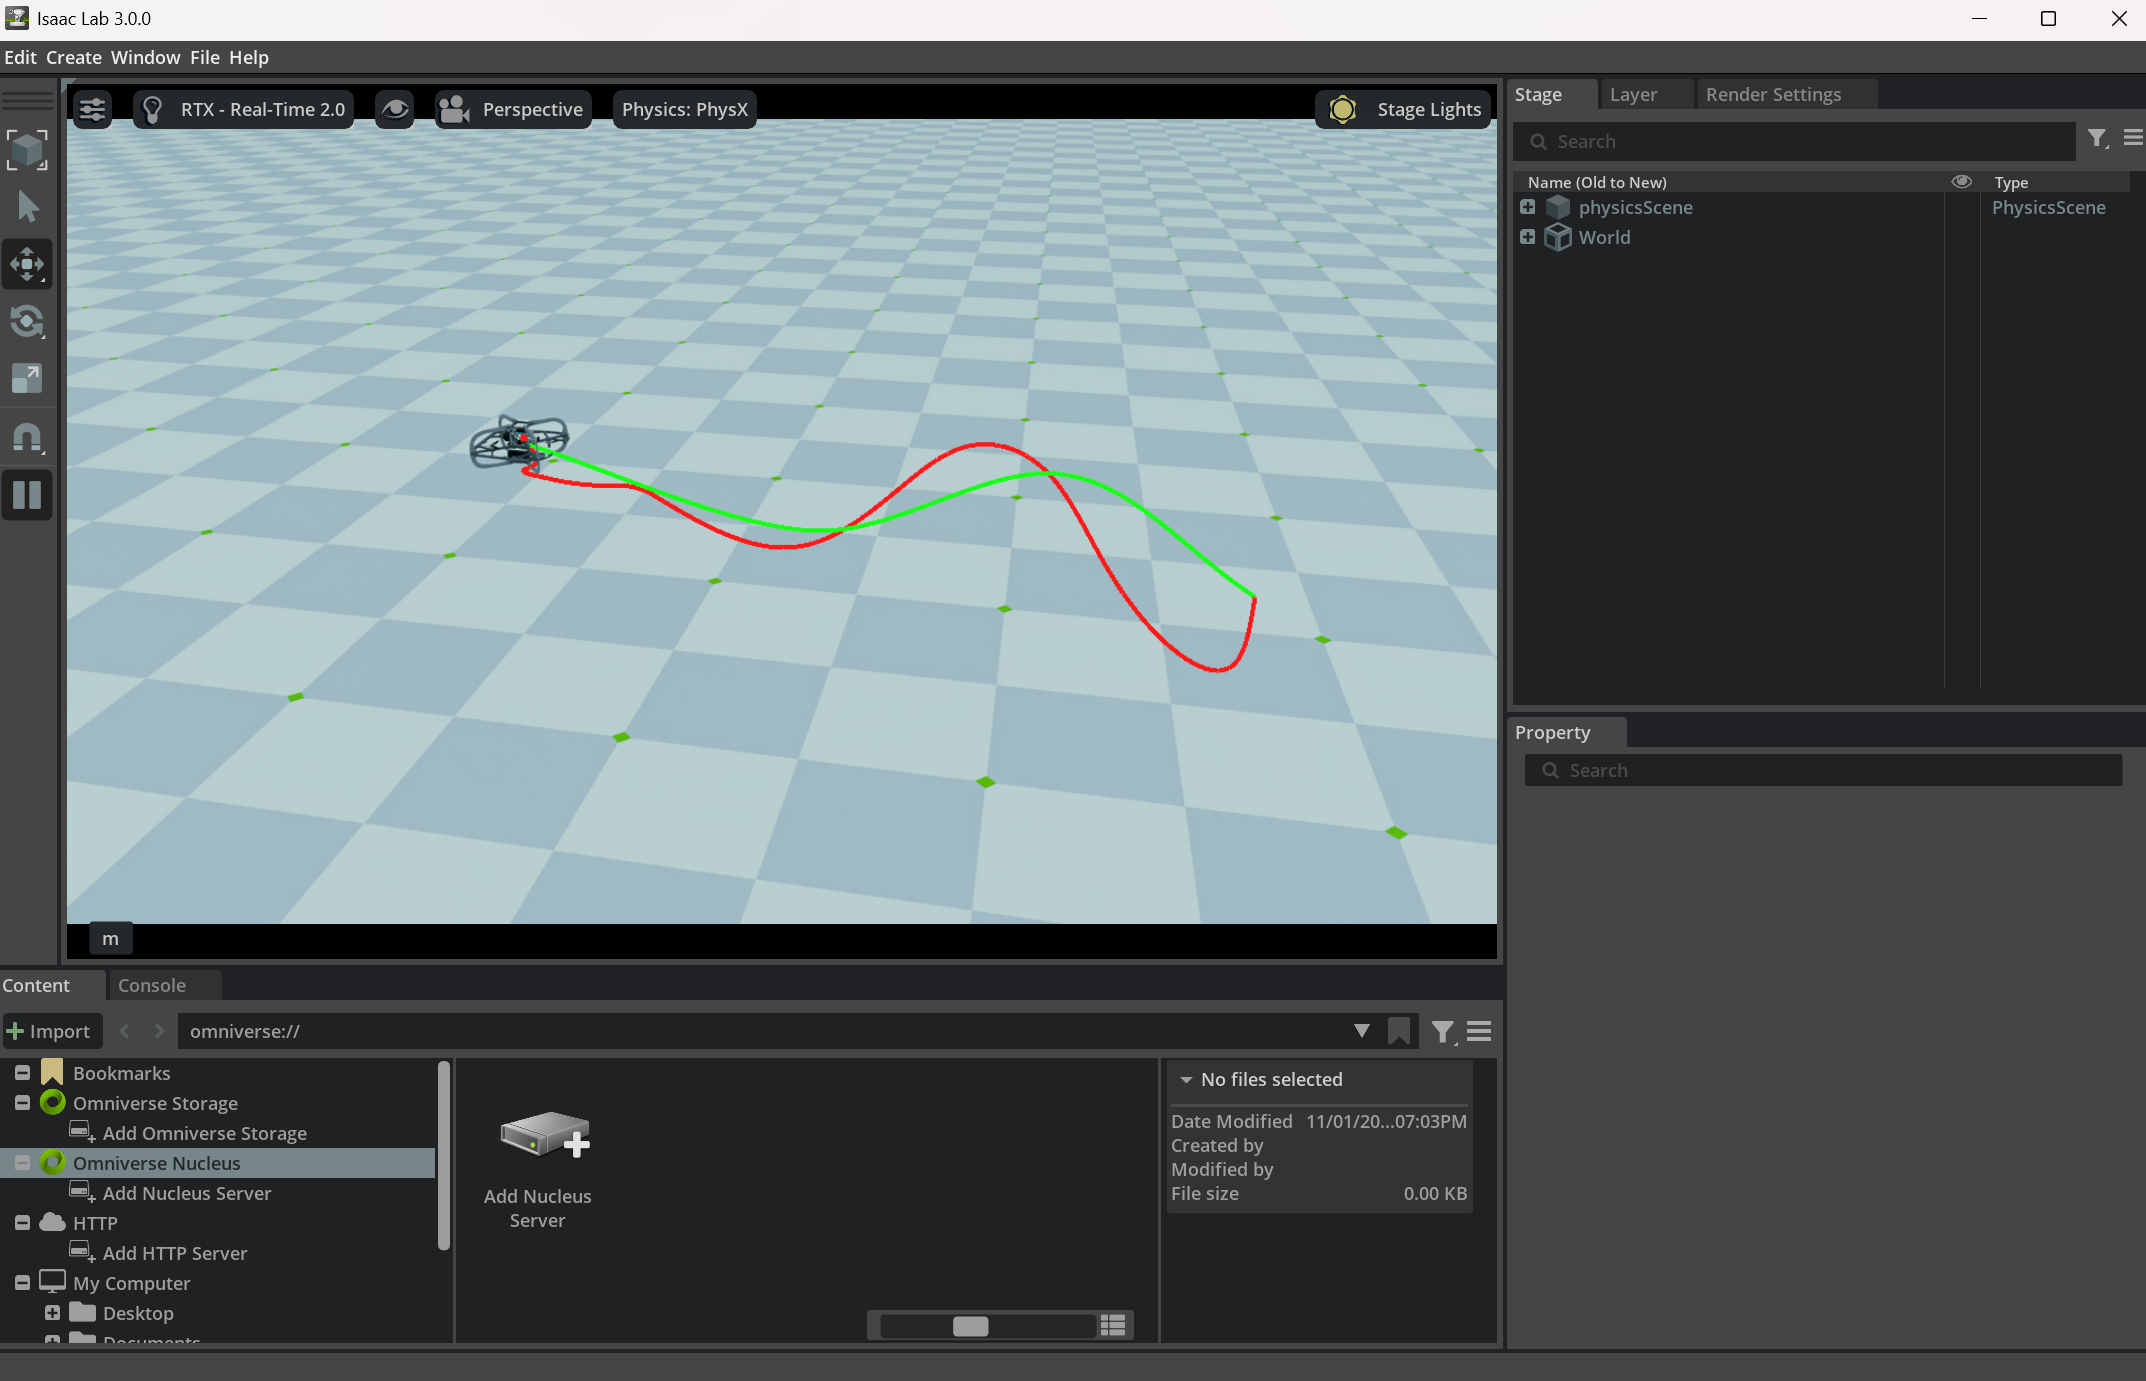
\includegraphics[width=0.8\linewidth]{figure/simexample.png}
    \caption{An example of a curved-path flight in Isaac Sim. The green path is the expected flight path and the red path is the actual flight path.}
    \label{fig:sim-example}
\end{figure}

The learned controllers operate using only sensory information that would be available to a real drone during flight. This includes the drone's motion, orientation, noisy IMU measurements, relative position and velocity to the target, and previous motor commands. The complete set of 26 input values is listed in Table \ref{tab:policy-inputs}.

\begin{table}[htbp]
\caption{The 26 values the learned policies observe at each step}
\label{tab:policy-inputs}
\resizebox{0.7\linewidth}{!}{\centering
\begin{tabular}{lll}
  \toprule
  Group    & Description                                 & Size \\
  \midrule
  Target   & Target position relative to the drone (m)   & 3 \\
           & Target velocity relative to the drone (m/s) & 3 \\
  State    & Drone velocity (m/s)                        & 3 \\
           & Orientation (quaternion)                    & 4 \\
           & Angular velocity (rad/s)                    & 3 \\
  IMU      & Accelerometer, noisy (m/s$^2$)              & 3 \\
           & Gyroscope, noisy (rad/s)                    & 3 \\
  Action   & Last thrust command per motor (N)           & 4 \\
  \midrule
  Total    &                                             & 26 \\
  \bottomrule
\end{tabular}}
\end{table}

With this methodology of comparing these controllers on the same flights, we aim to show not only whether a learned correction helps a drone survive a failing motor, but also at which fault sizes it is needed, how much recent flight history it requires, and when a carefully built PID is already enough.

\section{Methods}

\section{Results}

\section{Discussion}

\section{Conclusion}

\bibliography{reference}
\bibliographystyle{style/dsc180bibstyle}

\clearpage
\makeappendix

\subsection{AI Usage Disclosure}
We used AI assistants (Claude Opus 5.5, Claude Sonnet 5.5 and GPT 6.1 Sol) as coding agents. They drafted most of the code, tests and documentation, helped with debugging, and suggested wording edits to this report. The research questions, experiment design, literature review, analysis and conclusions are our own. At least one team member reviewed every AI-generated change. Code changes were also verified with unit tests and simulation runs before we kept them. Our tools, review process and major prompts are documented in \texttt{AI\_USE.md} in our repository:

\url{https://github.com/j2doan/drone-degradation-control}.

\end{document}